%\documentclass[xcolor=dvipsnames , 9pt]{beamer} 
%\usetheme{Copenhagen} 
%
%%%%%%%%%%%%%%%%%
%
%\usepackage{concrete}
%\usepackage{fancybox}
%\usepackage{amsmath}
%\usepackage{color, colortbl}
%\usepackage{array,arydshln}
%\usepackage{graphicx}
%\usepackage{subfig}
%\usepackage{caption}
%\usepackage{multirow}
%\usepackage{amsmath,amssymb}
%\usepackage{mathptm}
%\usepackage{verbatim}
%\usepackage[english]{babel}
%\usepackage{algorithm2e}
%\usepackage{fancybox}
%\usepackage{tikz}
%\usetikzlibrary{decorations.pathreplacing,angles,quotes}
%\usepackage{mathtools}
%\usepackage{subfig}
%\usepackage{color}
%\usepackage{mathtools}
%\usefonttheme{serif}
%%\newcommand\Nfont{\fontsize{9}{7.2}\selectfont}

\documentclass{beamer}




\usepackage{rotating}
\usepackage{tabularx}
\usepackage{multicol, blindtext}
\usepackage{subcaption}

\usepackage[T1]{fontenc}
\usepackage{graphicx} % http://ctan.org/pkg/graphicx
\usepackage{booktabs} % http://ctan.org/pkg/booktabs
\usepackage{xparse}
\usepackage{mdframed}
\usepackage{framed}
\usepackage{cuted}

\usepackage{tikz}
\usepackage{adjustbox}
\usepackage{tikz-cd}
\usetikzlibrary{decorations.markings}
\tikzset{negated/.style={
		decoration={markings,
			mark= at position 0.5 with {
				\node[transform shape] (tempnode) {$\backslash$};
			}
		},
		postaction={decorate}
	}
}

\usepackage{mathtools}
\DeclarePairedDelimiter{\ceil}{\lceil}{\rceil}




\renewenvironment{framed}[1][\hsize]
{\MakeFramed{\hsize#1\advance\hsize-\width \FrameRestore}}%
{\endMakeFramed}

\newcolumntype{C}[1]{>{\centering\let\newline\\\arraybackslash\hspace{0pt}}m{#1}}

\NewDocumentCommand{\rot}{O{90} O{1em} m}{\makebox[#2][l]{\rotatebox{#1}{#3}}}

\newcommand{\specialcell}[2][c]{%
	\begin{tabular}[#1]{@{}c@{}}#2\end{tabular}}
\newcommand{\Dim}{\textrm{Dim}}
\usepackage{rotating}
\usepackage{adjustbox}
\usepackage{tikz-cd}
\usepackage{subcaption}
\mode<presentation> {
	
	% The Beamer class comes with a number of default slide themes
	% which change the colors and layouts of slides. Below this is a list
	% of all the themes, uncomment each in turn to see what they look like.
	
	%\usetheme{default}
	%\usetheme{AnnArbor}
	%\usetheme{Antibes}
	%\usetheme{Bergen}
	%\usetheme{Berkeley}
	%\usetheme{Berlin}
	%\usetheme{Boadilla}
	%\usetheme{CambridgeUS}
	\usetheme{Copenhagen}
	%\usetheme{Darmstadt}
	%\usetheme{Dresden}
	%\usetheme{Frankfurt}
	%\usetheme{Goettingen}
	%\usetheme{Hannover}
	%\usetheme{Ilmenau}
	%\usetheme{JuanLesPins}
	%\usetheme{Luebeck}
%	\usetheme{Madrid}
	%\usetheme{Malmoe}
	%\usetheme{Marburg}
	%\usetheme{Montpellier}
	%\usetheme{PaloAlto}
	%\usetheme{Pittsburgh}
	%\usetheme{Rochester}
	%\usetheme{Singapore}
	%\usetheme{Szeged}
	%\usetheme{Warsaw}
	
	% As well as themes, the Beamer class has a number of color themes
	% for any slide theme. Uncomment each of these in turn to see how it
	% changes the colors of your current slide theme.
	
	%\usecolortheme{albatross}
	%\usecolortheme{beaver}
	%\usecolortheme{beetle}
	%\usecolortheme{crane}
	%\usecolortheme{dolphin}
	%\usecolortheme{dove}
	%\usecolortheme{fly}
	%\usecolortheme{lily}
	%\usecolortheme{orchid}
	%\usecolortheme{rose}
	%\usecolortheme{seagull}
	%\usecolortheme{seahorse}
	%\usecolortheme{whale}
	%\usecolortheme{wolverine}
	
	%\setbeamertemplate{footline} % To remove the footer line in all slides uncomment this line
	%\setbeamertemplate{footline}[page number] % To replace the footer line in all slides with a simple slide count uncomment this line
	
	%\setbeamertemplate{navigation symbols}{} % To remove the navigation symbols from the bottom of all slides uncomment this line
}
%\usepackage[usenames,dvipsnames]{xcolor}
\usepackage{graphicx} % Allows including images
\usepackage{booktabs} % Allows the use of \toprule, \midrule and \bottomrule in tables
\usepackage{tikz}
\usetikzlibrary{decorations.pathreplacing,angles,quotes}
\usepackage{caption}

\usepackage{float}

\newcommand*\circled[1]{\tikz[baseline=(char.base)]{% <---- BEWARE
		\node[shape=circle,draw,inner sep=2pt] (char) {#1};}}
%\usepackage[noae]{Sweave}
%\usepackage{helvet}

\defbeamertemplate*{footline}{shadow theme}{%
\leavevmode%
\hbox{\begin{beamercolorbox}[wd=.5\paperwidth,ht=2.5ex,dp=1.125ex,leftskip=.3cm plus1fil,rightskip=.3cm]{author in head/foot}%
    \usebeamerfont{author in head/foot}\hfill\insertshortauthor
\end{beamercolorbox}%

\begin{beamercolorbox}[wd=.5\paperwidth,ht=2.5ex,dp=1.125ex,leftskip=.3cm,rightskip=.3cm plus1fil]{title in head/foot}%
    \usebeamerfont{title in head/foot}\insertshorttitle\hfill%
\insertframenumber\,/\,\inserttotalframenumber
\end{beamercolorbox}}%
\vskip0pt%
}
%%%%%%%%%%%%%%%%

\title{
Digital signature from I-PLWE
}

%\subtitle{a measure on matchings}


% {\tt m.pourpouneh@ut.ac.ir}
%\vspace{3mm}
%Supervisor:\\
%Shahram Khazaei

\date{}

%%%%%%%%%%%%%%%%

\AtBeginSection[]{
	\begin{frame}
		\vfill
		\centering
		\begin{beamercolorbox}[sep=8pt,center,shadow=true,rounded=true]{title}
			\usebeamerfont{title}\insertsectionhead\par%
		\end{beamercolorbox}
		\vfill
	\end{frame}
}


%===========================================
\usepackage{svg}
\usepackage{rotating}
\usepackage{tabularx}
\usepackage{multicol, blindtext}
\usepackage{subcaption}
\usepackage{mdframed}
\usepackage{framed}
\usepackage{cuted}
\usepackage{tikz}
\usepackage{adjustbox}
\usepackage{tikz-cd}
\usetikzlibrary{decorations.markings}
\tikzset{negated/.style={
		decoration={markings,
			mark= at position 0.5 with {
				\node[transform shape] (tempnode) {$\backslash$};
			}
		},
		postaction={decorate}
	}
}
\usepackage[T1]{fontenc}
\usepackage{graphicx}
\usepackage{epstopdf}
% http://ctan.org/pkg/graphicx
\usepackage{booktabs} % http://ctan.org/pkg/booktabs
\usepackage{xparse}
\usepackage{mdframed}
\usepackage{framed}
\usepackage{cuted}

\usepackage{mathtools}
%\DeclarePairedDelimiter{\ceil}{\lceil}{\rceil}


\renewenvironment{framed}[1][\hsize]
{\MakeFramed{\hsize#1\advance\hsize-\width \FrameRestore}}%
{\endMakeFramed}

\newcolumntype{C}[1]{>{\centering\let\newline\\\arraybackslash\hspace{0pt}}m{#1}}

%\NewDocumentCommand{\rot}{O{90} O{1em} m}{\makebox[#2][l]{\rotatebox{#1}{#3}}}

%\newcommand{\specialcell}[2][c]{%
%	\begin{tabular}[#1]{@{}c@{}}#2\end{tabular}}


\newcommand{\listqh}{\mathcal{I}}


%\newcommand{\MonL}[1]{\mathsf{Leak}_{\textsc{Mon}}^{#1}}
\newcommand{\MonL}[1]{\mathsf{MonLeak}_{#1}}
\newcommand{\MinL}{\mathsf{MinLeak}}
%\newcommand{\ML}{\mathsf{Leak}_{\textsc{LH}}}
\newcommand{\ML}{\mathsf{LeakLH}}
%\newcommand{\WML}{\mathsf{Leak}_{\textsc{LL}}}
\newcommand{\WML}{\mathsf{LeakLL}}

\newcommand{\distribution}{\mathcal{D}}
\newcommand{\completion}{\mathcal{C}}
\newcommand{\groupset}{\mathcal{GS}}

\newcommand{\Size}{\textrm{Size}}
\newcommand{\OPP}{\textrm{OPP}}
\newcommand{\opq}{\mathrm{O}}
\newcommand{\To}{\textbf{ to }}
\newcommand{\cmac}{\textsc{MAC}}
\newcommand{\gen}{\mathsf{Gen}}
\newcommand{\mac}{\mathsf{Mac}}
\newcommand{\vrfy}{\mathsf{Vrfy}}
\newcommand{\adv}{\mathsf{Adv}}
\newcommand{\partsec}{3Partition}
\newcommand{\lpar}{\mathsf{M3P}}

\newcommand{\partt}{\mathsf{3P}}

\newcommand{\indsec}{\mathsf{aIND}}
\newcommand{\cdb}{\mathsf{ConstructDB}}
\newcommand{\adjoin}{\mathsf{Adjoin}}
\newcommand{\nadjoin}{\text{Adjoin}}
\newcommand{\adjust}{\mathsf{Adjust}}
\newcommand{\rnd}{\mathsf{Rand}}
\newcommand{\addclm}{\mathsf{Addlbl}}
\newcommand{\expr}{\mathsf{Exp}}
\newcommand{\advvd}{\mathcal{D}}
\newcommand{\chal}{\mathsf{Chal}}

%----------------------- Notation -----------------------------------
\newcommand{\ds}{\mathcal{DS}}
\newcommand{\ul}{\mathcal{L}}
\newcommand{\db}{\mathcal{DB}}
\newcommand{\indi}{lbl_i}
\newcommand{\indl}{l}
\newcommand{\ind}{\mathcal{L}}
\newcommand{\setclm}{\mathcal{C}}
\newcommand{\set}{S}
\newcommand{\universal}{\mathcal{W}}
\newcommand{\op}{op}
\newcommand{\q}{q}
\newcommand{\field}{\mathbb{F}}
\newcommand{\grp}{\mathbb{G}}
\newcommand{\zgrp}{\mathbb{Z}}
\newcommand{\gengrp}{\mathcal{G}}
\newcommand{\nature}{\mathbb{N}}
\newcommand{\convert}{\mathsf{Convert}}
\newcommand{\rf}{RF}
\newcommand{\tprf}{\text{PRF}}
\newcommand{\btprf}{\mathsf{PRF}}
\newcommand{\oracle}{\mathcal{O}}
\newcommand{\intersec}{\boldsymbol{\cap}}
\newcommand{\union}{\boldsymbol{\cup}}
\newcommand{\diff}{\boldsymbol{\setminus}}
\newcommand{\mmship}{\boldsymbol{\in}}
\newcommand{\pso}{\mathsf{PSO}}
\newcommand{\npso}{\text{PSO}}
\newcommand{\ntset}{\text{Tset}}
\newcommand{\psii}{\mathsf{PSI}}
\newcommand{\psu}{\mathsf{PSU}}
\newcommand{\psize}{N}
\newcommand{\mparam}{m}
\newcommand{\nparam}{n}
\newcommand{\mH}{{\mathcal H}}
%----------------------- Def. Scheme  -----------------------------
\newcommand{\sosse}{\mathsf{PSO}}
\newcommand{\keygen}{\mathsf{Gen}}
\newcommand{\edssetup}{\mathsf{Enc}}
\newcommand{\token}{\mathsf{Token}}
\newcommand{\search}{\mathsf{Oprate}}
\newcommand{\retrive}{\mathsf{Retrieve}}
\newcommand{\sk}{K}
\newcommand{\ot}{sot}
\newcommand{\skl}{k}
\newcommand{\eds}{\widetilde{\mathcal{DS}}}
\newcommand{\edb}{EDB}
\newcommand{\edc}{\widetilde{D}}
\newcommand{\tk}{tk}
\newcommand{\eelm}{\widetilde{S}}
\newcommand{\elm}{S}
\newcommand{\nske}{\text{SKE}}
\newcommand{\ske}{\mathsf{SKE}}
\newcommand{\init}{\mathsf{Initialize}}
\newcommand{\tset}{\mathsf{Tset}}
\newcommand{\tkeygen}{\mathsf{Gen}}
\newcommand{\tsetup}{\mathsf{Hash}}
\newcommand{\ttag}{\mathsf{Token}}
\newcommand{\tretrive}{\mathsf{Retrive}}
\newcommand{\qg}{Q}
\newcommand{\stag}{rt}
\newcommand{\eset}{\widetilde{\tarray}}
\newcommand{\tarray}{\mathcal{T}}
\newcommand{\resset}{S}
%----------------------- Construction -----------------------------
\newcommand{\oxt}{\mathsf{OXT}}
\newcommand{\sparam}{S}
\newcommand{\bparam}{B}
\newcommand{\free}{Free}
\newcommand{\record}{Record}
\newcommand{\skg}{sk}
\newcommand{\groupgen}{\mathsf{GroupGen}}
\newcommand{\prfa}{F}
\newcommand{\f}{f}
\newcommand{\g}{g}
\newcommand{\prfb}{\tilde{F}}
\newcommand{\skenc}{\mathsf{Enc}}
\newcommand{\adjenc}{\mathsf{Encod}}
\newcommand{\share}{\mathsf{Share}}
\newcommand{\reconstruct}{\mathsf{Recovery}}
\newcommand{\dec}{\mathsf{Dec}}
\newcommand{\ekeygen}{\mathsf{\Pi.KeyGen}}
\newcommand{\penc}{\mathsf{Enc}}
\newcommand{\pdec}{\mathsf{Dec}}
\newcommand{\pkeygen}{\mathsf{Gen}}
\newcommand{\Z}{\mathbb{Z}}
%----------------------- Security Def. -----------------------------
\newcommand{\advv}{\mathcal{A}}
\newcommand{\advvb}{\mathcal{B}}
\newcommand{\cor}{\mathsf{Cor}}
\newcommand{\prf}{\textsc{prf}}
\newcommand{\advantage}{\mathsf{Adv}}
\newcommand{\simv}{\mathcal{S}}
\newcommand{\realexp}{\mathsf{Real}}
\newcommand{\nasim}{\mathsf{naSIM}}
\newcommand{\ideal}{\mathsf{Ideal}}
\newcommand{\Leakage}{\mathcal{L}}
\newcommand{\ngl}{\mathsf{negl}}
\newcommand{\cpa}{\textsc{CPA}}
\newcommand{\bcpa}{\mathsf{CPA}}
\newcommand{\ddh}{\mathsf{DDH}}
\newcommand{\searchp}{SP}
\newcommand{\resultp}{RP}
\newcommand{\sizep}{SS}
\newcommand{\opg}{OP}
\newcommand{\indg}{IND}
\newcommand{\N}{N}
%\newcommand{\N}{\mathbb{N}}
\newcommand{\tsetcor}{\mathsf{TSetCor}}
%----------------------- Security Proof -----------------------------
\newcommand{\tkg}{TK}
\newcommand{\res}{S}
\newcommand{\reset}{RS}
\newcommand{\stg}{ST}
\newcommand{\adjg}{ADJ}
\newcommand{\adj}{Adj}
\newcommand{\addj}{\mathsf{ADJUST}}
\newcommand{\initialize}{\mathsf{Initialize}}
\newcommand{\game}{\mathsf{Game}}
\newcommand{\simul}{\mathsf{Simulator}}
\newcommand{\rfa}{\hat{f}}
%----------------------- miscellaneous -----------------------------
\newcommand{\Gen}{\mathsf{Setup}}
\newcommand{\Index}{\mathsf{BuildIndex}}
\newcommand{\Token}{\mathsf{Token}}
\newcommand{\Tag}{\mathsf{Tag}}
\newcommand{\Search}{\mathsf{Search}}
\newcommand{\Retrieve}{\mathsf{Retrieve}}
\newcommand{\Verif}{\mathsf{PubVerif}}
\newcommand{\secparam}{\lambda}
\newcommand{\expsecparam}{1^\secparam}
\newcommand{\SK}{k}
\newcommand{\Doccol}{\mathcal{D}}
\newcommand{\IndexD}{\mathcal{I}}
\newcommand{\Masspace}{\mathcal{M}}
\newcommand{\keyspace}{K}
\newcommand{\wordspace}{W}
\newcommand{\docid}{ID}
\newcommand{\Sim}{S}
\newcommand{\Prob}{\Pr}
\newcommand{\Simw}{\mathsf{Sim}}
\newcommand{\Realw}{\mathsf{Real}}
\newcommand{\ndoc}{n}
\newcommand{\nuser}{m}
\newcommand{\useri}{{U}_i}
\newcommand{\Cset}{\mathcal{C}}
\newcommand{\dcol}{\mathcal{D}}
\newcommand{\AG}{\mathcal{G}}
\newcommand{\edgAG}{E(\mathcal{G})}
\newcommand{\edg}{E}
\newcommand{\uk}{uk}
\newcommand{\dk}{k}
\newcommand{\owner}{D.O}
\newcommand{\docj}{D_j}
\newcommand{\ser}{Ser}
\newcommand{\uki}{uk_i}
\newcommand{\dkj}{k_j}
\newcommand{\HF}{H}
\newcommand{\sHF}{H_2}
\newcommand{\fg}{G_1}
\newcommand{\sg}{G_2}
\newcommand{\tg}{G_T}
\newcommand{\bm}{e}
\newcommand{\kw}{w}
\newcommand{\random}{r}
\newcommand{\eqDeltaij}{\Delta(\uki,\dkj)=g_2^{\frac{\dkj}{\uki}}}
\newcommand{\eqencj}{<\random,\sHF(\random,\bm(\HF(\kw),g_2)^{\dkj})>}
\newcommand{\eqtokeni}{\HF^{\uki}(\kw)}
\newcommand{\Deltaij}{\Delta(\uki,\dkj)}
\newcommand{\F}{F_{MKSE}}
\newcommand{\crupt}{\mathcal{C}}
\newcommand{\AP}{\mathcal{AP}}
\newcommand{\modifAP}{\AP^{m}}
\newcommand{\APi}{\AP_i}
\newcommand{\user}{\mathcal{U}}
\newcommand{\doc}{\mathcal{D}}
\newcommand{\dic}{\mathcal{W}}
%\newcommand{\indj}{ind_j}
\newcommand{\Setup}{Setup(1^{\secparam})}

\usepackage{threeparttable} 

\usepackage{amssymb,amsmath}
\usepackage{algpseudocode} 
\usepackage{algorithm}
\usepackage{adjustbox}
\usepackage{multirow}
\usepackage{tikz}
\usepackage{siunitx}
\sisetup{bracket-negative-numbers, open-bracket={
		{}^-% your custom hack here
	}, close-bracket={}}
%\newcommand*\circled[1]{\tikz[baseline=(char.base)]{
%		\node[shape=circle,draw,inner sep=0.5pt] (char) {#1};}}


\makeatletter
\newenvironment{breakablealgorithm}
{% \begin{breakablealgorithm}
	\begin{center}
		\refstepcounter{algorithm}% New algorithm
		\hrule height.8pt depth0pt \kern2pt% \@fs@pre for \@fs@ruled
		\renewcommand{\caption}[2][\relax]{% Make a new \caption
			{\raggedright\textbf{\ALG@name~\thealgorithm} ##2\par}%
			\ifx\relax##1\relax % #1 is \relax
			\addcontentsline{loa}{algorithm}{\protect\numberline{\thealgorithm}##2}%
			\else % #1 is not \relax
			\addcontentsline{loa}{algorithm}{\protect\numberline{\thealgorithm}##1}%
			\fi
			\kern2pt\hrule\kern2pt
		}
	}{% \end{breakablealgorithm}
		\kern2pt\hrule\relax% \@fs@post for \@fs@ruled
	\end{center}
}
\makeatother

\makeatletter
\newcommand*{\rom}[1]{\expandafter\@slowromancap\romannumeral #1@}
\makeatother

\newcommand{\univ}{\{0,1\}^\secparam}
\newcommand{\univs}{\big(\univ\big)^*}

\newcommand{\outl}{L}
\newcommand{\leak}{\mathsf{Leak}}

\newcommand{\listq}{\mathcal{Q}}
\newcommand{\listqi}{I_{\listq}}

\newcommand{\outlt}{L_T}
\newcommand{\leakt}{\mathsf{LeakT}}
\newcommand{\outla}{L_A}
\newcommand{\leaka}{\mathsf{LeakA}}
\newcommand{\outlp}{L_P}
\newcommand{\leakp}{\mathsf{LeakP}}
\newcommand{\poly}{\mathsf{poly}}
\newcommand{\inv}{\mathsf{Inv}}
\newcommand{\tbl}{\mathcal{T}}
\newcommand{\row}{R}
\newcommand{\clm}{C}
\newcommand{\at}{at}
\newcommand{\aew}{aw}
\newcommand{\dd}{D}


\usepackage{mathrsfs}
\newcommand{\otset}{\mathsf{Tset}}

\newcommand{\lft}{\mathscr{L}}
\newcommand{\mdl}{\mathscr{M}}
\newcommand{\rht}{\mathscr{R}}
%========================== BSSE
\newcommand{\nsse}{\text{SSE}}
\newcommand{\bsse}{\mathsf{BSSE}}
\newcommand{\nbsse}{\text{BSSE}}
\newcommand{\bsetup}{\mathsf{Enc}}
\newcommand{\bsearch}{\mathsf{Search}}

\newcommand{\bst}{bst}
\newcommand{\els}{\widetilde{L}}

\newcommand{\outlb}{L_B}
\newcommand{\leakb}{\mathsf{LeakB}}

\newcommand{\lbsse}{\mathsf{LeakB}}
\newcommand{\lpso}{\mathsf{LeakP}}

%========================== BSSE
%\newtheorem{struct_type}{struct_title}[in_counter]

\newtheorem{thm}{Theorem}

\newtheorem{convention}[thm]{\textit{Convention}}
%\newtheorem{Theorem}{\textit{Convention}}[convention]

%\newtheorem{assumption1}{Assumption}
\newtheorem{notation}{Notation}
\newtheorem{claim1}{Claim}

\newtheorem{proposition1}[thm]{Proposition}
\newtheorem{remark1}[thm]{Remark}
\newtheorem{definition1}[thm]{Definition}
\newtheorem{lemma1}[thm]{Lemma}
\newtheorem{corollary1}[thm]{Corollary}
\newtheorem{assumption1}[thm]{Assumption}
\newtheorem{example1}[thm]{Example}
\newtheorem{conjecture1}[thm]{Conjecture}

\usepackage{chngcntr}
%\counterwithin{theorem}{section}
%\counterwithin{proposition}{section}
%\counterwithin{corollary}{section}
%\counterwithin{definition}{section}
%\counterwithin{lemma}{section}
%\counterwithin{assumption}{section}
%\counterwithin{notation}{section}
%\counterwithin{claim1}{section}
%\counterwithin{remark}{section}
%\counterwithin{equation}{section}

\newcommand{\grt}{RT}
\newcommand{\gat}{AT}
\newcommand{\gbst}{BST}
\newcommand{\got}{SOT}

%==========================================================
\def\mymathhyphen{{\hbox{-}}}
\newcommand*{\backin}{\rotatebox[origin=c]{-180}{$\in$}}%

\newcommand{\nmadjoin}{\text{M-Adjoin}}
\newcommand{\ntss}{\text{TSS}}
\newcommand{\madjoin}{\Pi}%{\mathsf{M \mymathhyphen Adjoin}}
\newcommand{\parti}{\mathscr{L}}
\newcommand{\zpar}{\mathsf{M3P}}
\newcommand{\twopar}{\mathsf{2Par}}
\newcommand{\eval}{\mathsf{Eval}}
\newcommand{\listi}{\mathrm{I}}
\newcommand{\cindl}{lbl^c}
\newcommand{\naind}{\mathsf{naIND}}
\newcommand{\len}{m}
\newcommand{\asim}{\mathsf{aSIM}}
\newcommand{\setl}{\mathcal{L}}
\newcommand{\eq}{\mathrm{EQ}}
\newcommand{\ieq}{\mathrm{IEQ}}

\newcommand{\LBL}{\textrm{LBL}}
\newcommand{\aLBL}{\textrm{aLBL}}
\newcommand{\aDIM}{\textrm{aDIM}}
\newcommand{\aSP}{\textrm{aSP}}
\newcommand{\aDP}{\textrm{aDP}}
\newcommand{\DIM}{\textrm{DIM}}
\newcommand{\SP}{\textrm{SP}}
\newcommand{\DP}{\textrm{DP}}
\newcommand{\RP}{\textrm{RP}}
\newcommand{\aRP}{\textrm{aRP}}
\newcommand{\MP}{\textrm{MP}}

\newcommand{\MtP}{\text{M3P}}
\newcommand{\MtPK}{\text{M3P}_{$k$}}


\newcommand{\inds}{\texttt{IND}}
\newcommand{\ainds}{\texttt{aIND}}
\newcommand{\nainds}{\texttt{naIND}}
\newcommand{\aonainds}{\texttt{(n)aIND}}
\newcommand{\sims}{\texttt{SIM}}
\newcommand{\asims}{\texttt{aSIM}}
\newcommand{\nasims}{\texttt{naSIM}}


\newcommand{\tp}{\texttt{3Partition}}
\newcommand{\stp}{\texttt{3P}}
\newcommand{\mtp}{\texttt{M3Partition}}
\newcommand{\smtp}{\texttt{M3P}}
\newcommand{\mtpk}[1]{\smtp_{#1}}
\newcommand{\smtpk}[1]{\smtp_{#1}}


\newcommand{\sMtP}{\text{M3Partiotion}}
\newcommand{\sMtPk}{\text{M3Pasrtition_$k$}}

\let\ACMmaketitle=\maketitle
\renewcommand{\maketitle}{\begingroup\let\footnote=\thanks \ACMmaketitle\endgroup}

\newcommand{\lk}{lk}
\newcommand{\wk}{wk}
%\usepackage{graphicx}
\usepackage{hyperref}
\usepackage{pifont}
\newcommand{\cmark}{\ding{51}}%
\newcommand{\xmark}{\ding{53}}%
\usepackage{centernot}


\usepackage{filecontents}
%\usepackage[noadjust]{cite}
\usepackage{cite}

\usepackage{ragged2e}

% correct bad hyphenation here
\hyphenation{op-tical net-works semi-conduc-tor}

\usepackage[T1]{fontenc} 
\usepackage{graphicx}
\usepackage{epstopdf}

\def\NoNumber#1{{\def\alglinenumber##1{}\State#1}\addtocounter{ALG@line}{-1}}


\newcommand*\emptycirc[1][0.75ex]{\tikz\draw (0,0) circle (#1);} 
\newcommand*\halfcirc[1][0.75ex]{%
	\begin{tikzpicture}
	\draw[fill] (0,0)-- (90:#1) arc (90:270:#1) -- cycle ;
	\draw (0,0) circle (#1);
	\end{tikzpicture}}
\newcommand*\fullcirc[1][0.75ex]{\tikz\fill (0,0) circle (#1);}

\usepackage{forest}

\newenvironment{chapterFrame}[1]{%
	\begin{frame}[plain]
		\begin{block}{}\centering
			{\Huge Chapter \thesection}\par\medskip
			{\Large #1}
		\end{block}
%		\vfill\tableofcontents
	}{\end{frame}}

\newcommand{\Arrow}[1]{%
	\parbox{#1}{\tikz{\draw[->](0,0)--(#1,0);}}
}

\usepackage{setspace}



\begin{document}

%%%%%%%%%%%%%%%%%%%
\begin{frame}
\begin{figure}[h]
\centering

\includegraphics[scale=0.2]{logo}
\end{figure}

  \titlepage
\end{frame}
%%%%%%%%%%%%%%%%%%%
%\begin{frame}
%%  \frametitle{Contents}
%%%  \tableofcontents[shaded]
%%  \tableofcontents
%\end{frame}
%%%%%%%%%%%%%%%%%
% TABLE OF CONTENTS AT BEGIN OF EACH SECTION
%\AtBeginSection[]{
%  \begin{frame}<beamer>
%    \frametitle{Current Section}
%    \tableofcontents[currentsection]
%  \end{frame}}
%%%%%%%%%%%%%%%%%%%%%%%%%%%%%%%%%%%%%%%%%%%%%%%%%%%%%%%%%%%%%%%%%%%%%%%%%%%%

\begin{frame}{Table of Contents}

{\footnotesize\setstretch{1.75}
\begin{multicols}{2}
\tableofcontents
\end{multicols}	
}	
%	\begin{itemize}
%		\item Overview
%		\item Private Set Operation ($\npso$) Schemes,
%		\item Multi-Adjustable Join ($\nmadjoin$) Schemes,
%		\item $\nmadjoin$ Security Notions: Separations and implications.	 
%	\end{itemize}
\end{frame}
%%%%%%%%%%%%%%%%%%%%%%%%%%%%%%%%%%%%%%%%%%%%%%%%%%%%%%%%%%%%%%%%%%%%%%%%%%%%


%=============================== SECTION 1 ===================================

\section{Ring LWE}

\begin{frame}{Ring LWE}
	\begin{minipage}{0.42\linewidth}
		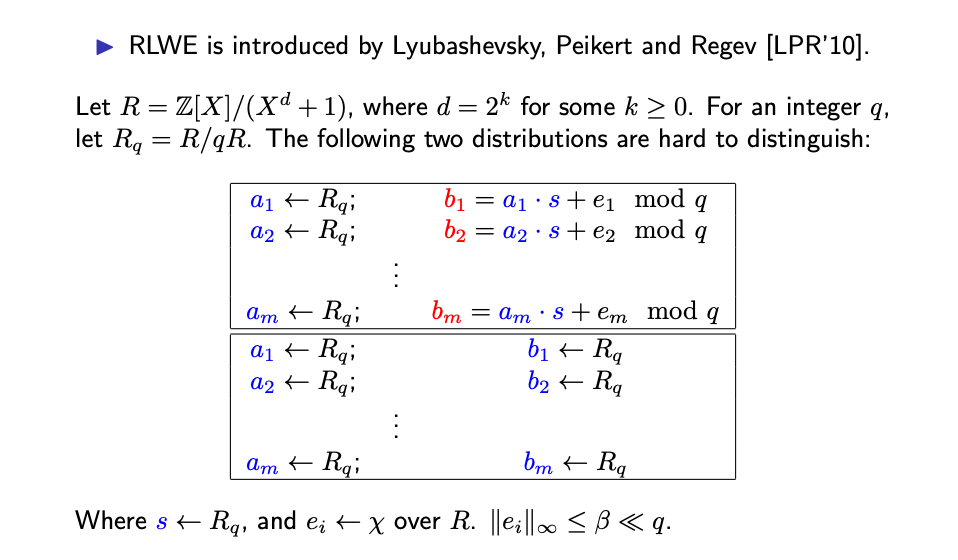
\includegraphics[scale=0.65]{1.png}
	\end{minipage}
\end{frame}

\begin{frame}{Ring LWE}
	\begin{minipage}{0.42\linewidth}
		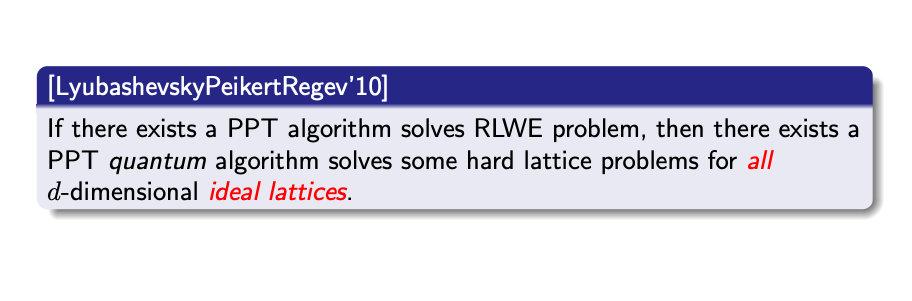
\includegraphics[scale=0.65]{2.png}
	\end{minipage}
\end{frame}

\section{Commitment scheme}

\begin{frame}{Commitment scheme}
	\begin{minipage}{0.42\linewidth}
		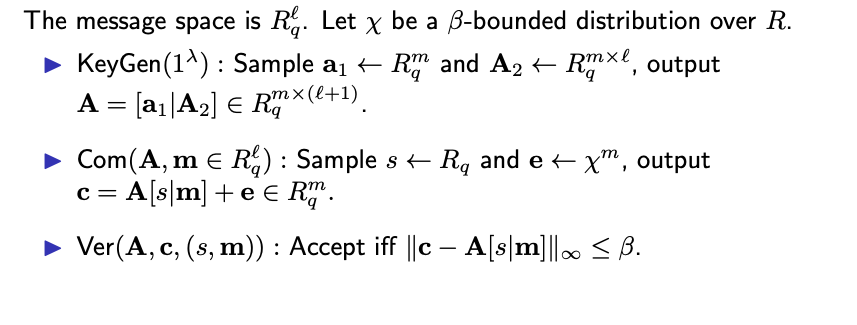
\includegraphics[scale=0.65]{3.png}
	\end{minipage}
\newline
\newline
Is $e$ going to be $\beta$ bounded when we replace $e$ with $e(q)$ ?
\end{frame}

\begin{frame}{Commitment scheme}
	\begin{minipage}{0.42\linewidth}
		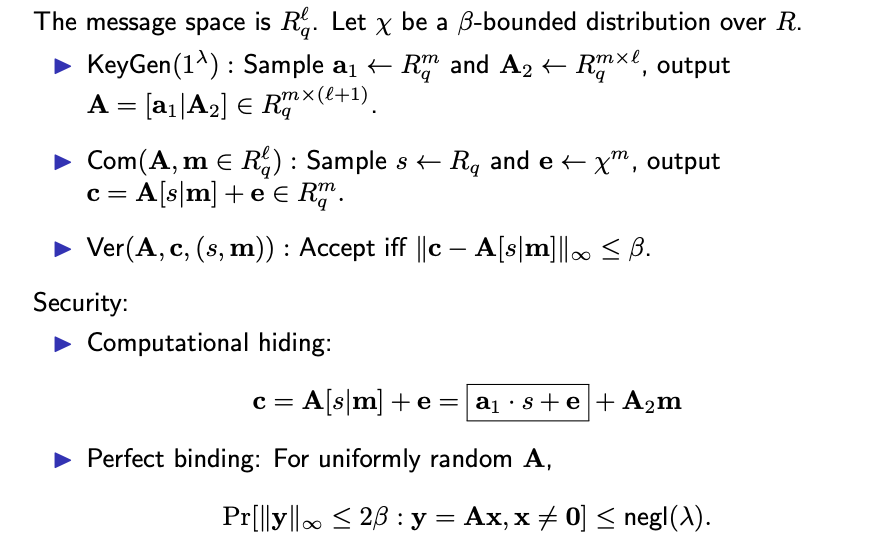
\includegraphics[scale=0.65]{4.png}
	\end{minipage}
\end{frame}

\subsection{issues}

\begin{frame}{issues}
	\begin{minipage}{0.42\linewidth}
		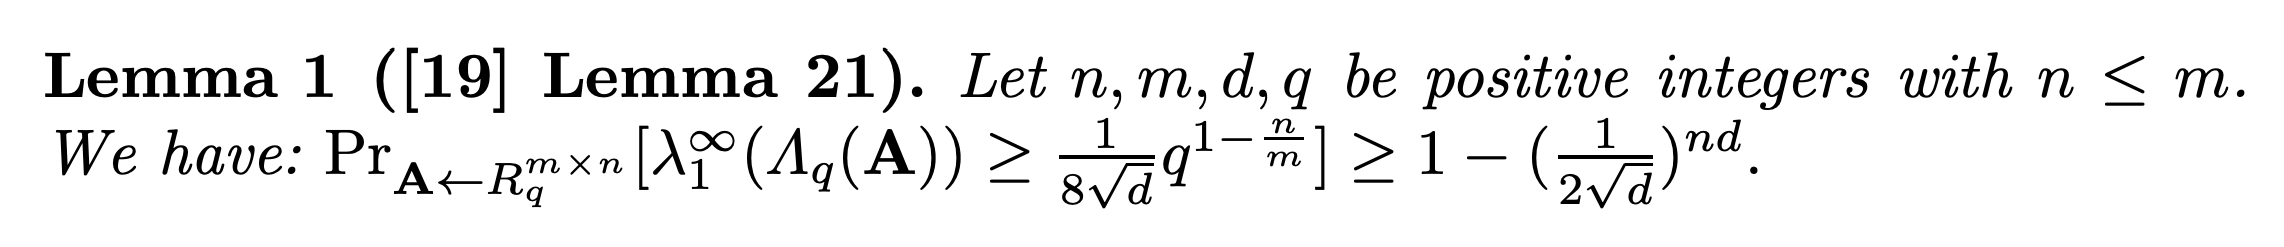
\includegraphics[scale=0.25]{i1.png}
	\end{minipage}
\newline
\newline
\newline
Is this lemma true when we replace a polynomial with a value?
\end{frame}

\section{Zero knowledge proof}

\begin{frame}{Zero knowledge proof}
	\begin{minipage}{0.42\linewidth}
		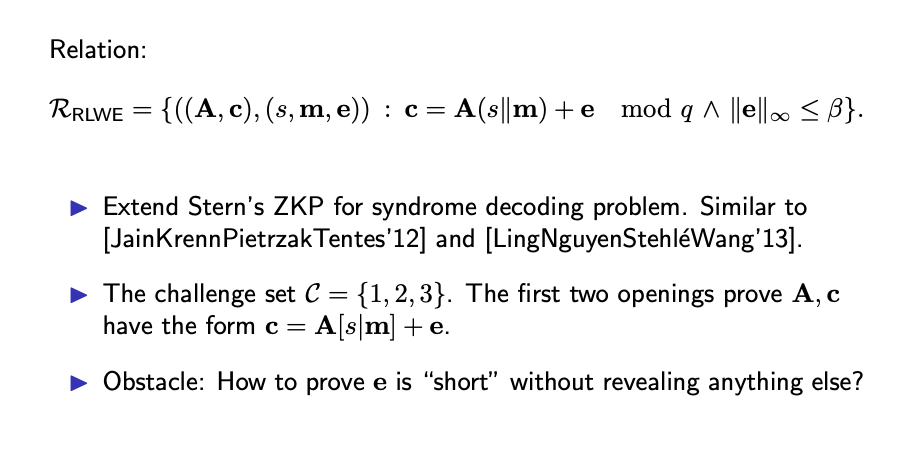
\includegraphics[scale=0.65]{5.png}
	\end{minipage}
\end{frame}



\begin{frame}{Zero knowledge proof}
	\begin{minipage}{0.42\linewidth}
		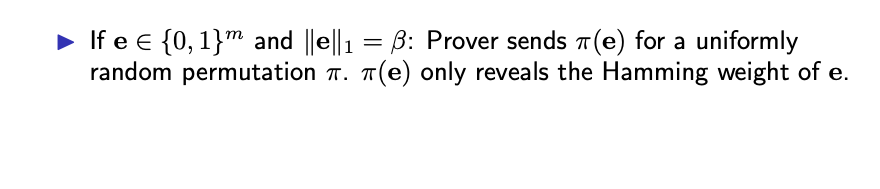
\includegraphics[scale=0.65]{6.png}
	\end{minipage}
\end{frame}


\begin{frame}{Zero knowledge proof}
	\begin{minipage}{0.42\linewidth}
		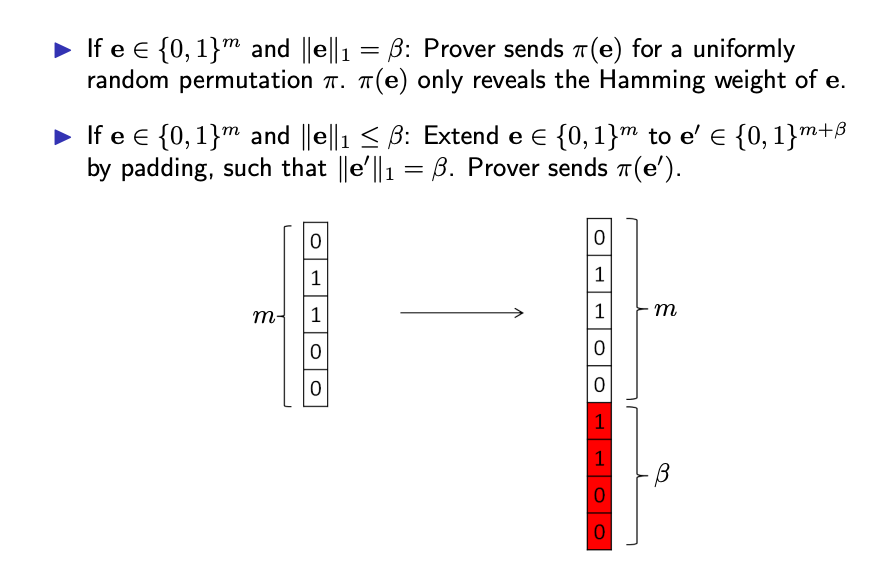
\includegraphics[scale=0.65]{7.png}
	\end{minipage}
\end{frame}

\begin{frame}{Zero knowledge proof}
	\begin{minipage}{0.42\linewidth}
		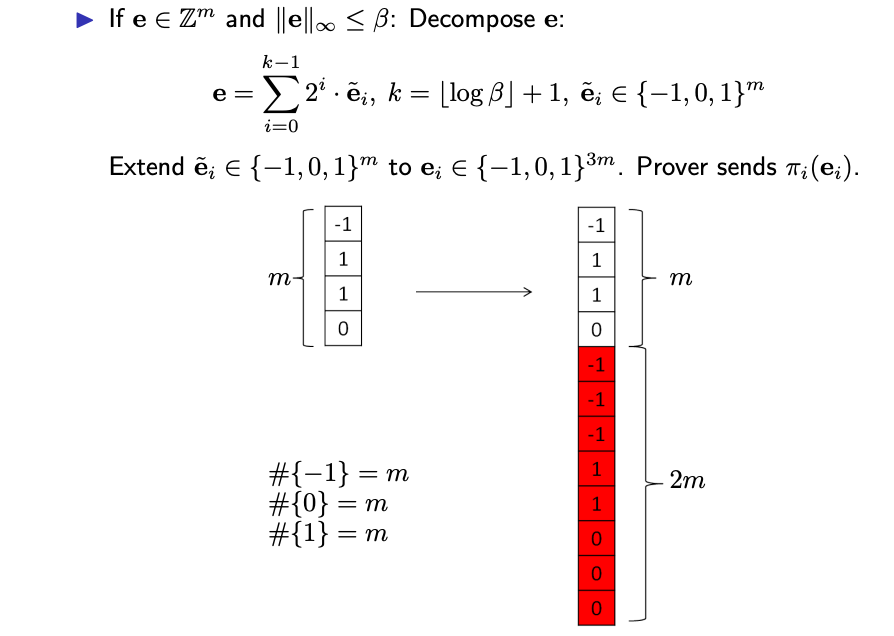
\includegraphics[scale=0.65]{8.png}
	\end{minipage}
\end{frame}

\begin{frame}{Zero knowledge proof}
	\begin{minipage}{0.42\linewidth}
		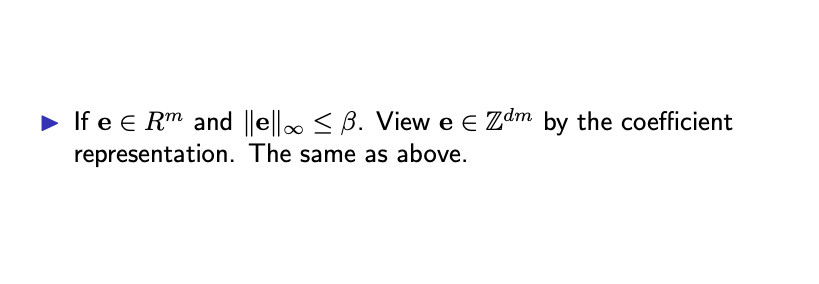
\includegraphics[scale=0.65]{9.png}
	\end{minipage}
\end{frame}

\begin{frame}{Zero knowledge proof}
	\begin{minipage}{0.42\linewidth}
		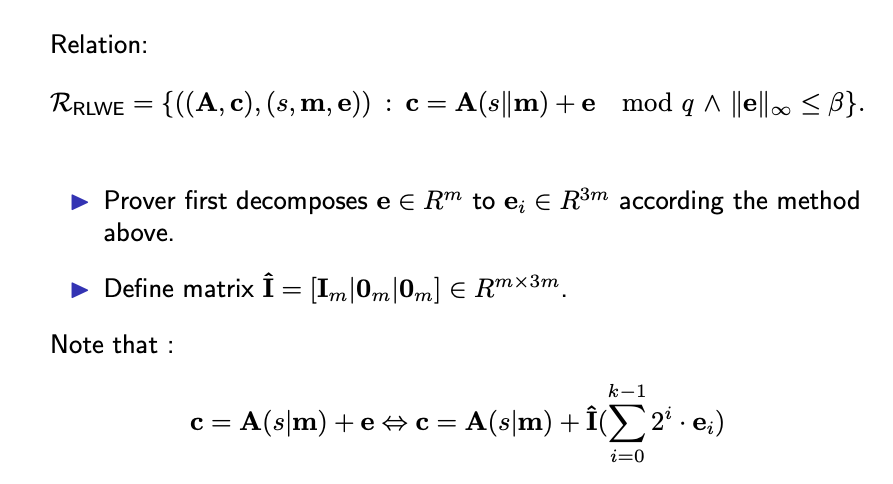
\includegraphics[scale=0.65]{10.png}
	\end{minipage}
\end{frame}

\begin{frame}{Zero knowledge proof}
	\begin{minipage}{0.42\linewidth}
		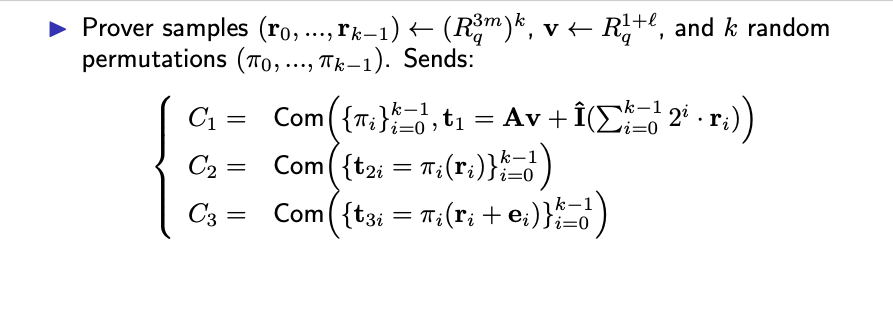
\includegraphics[scale=0.65]{11.png}
	\end{minipage}
\end{frame}

\begin{frame}{Zero knowledge proof}
	\begin{minipage}{0.42\linewidth}
		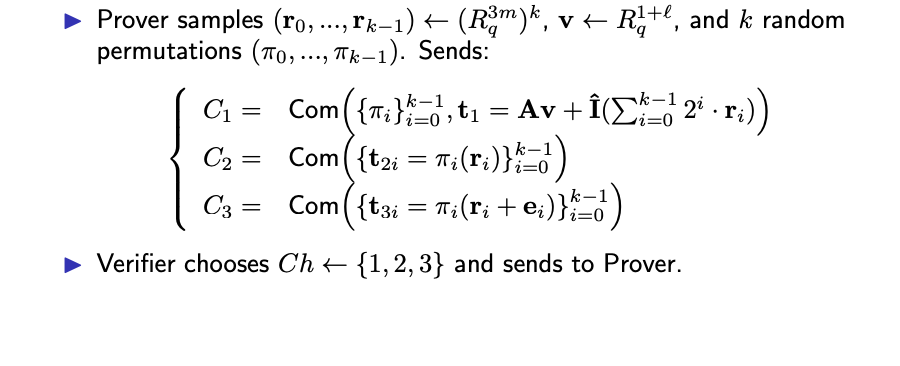
\includegraphics[scale=0.65]{12.png}
	\end{minipage}
\end{frame}

\begin{frame}{Zero knowledge proof}
	\begin{minipage}{0.42\linewidth}
		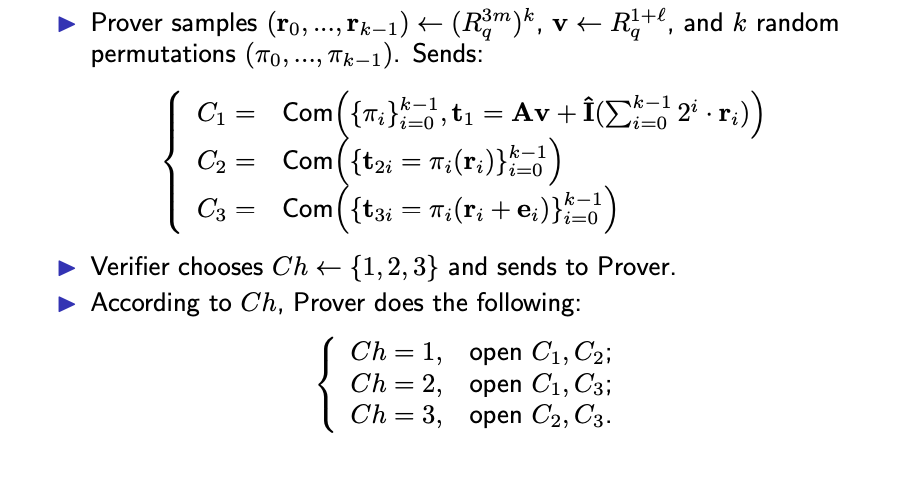
\includegraphics[scale=0.65]{13.png}
	\end{minipage}
\end{frame}

\begin{frame}{Zero knowledge proof}
	\begin{minipage}{0.42\linewidth}
		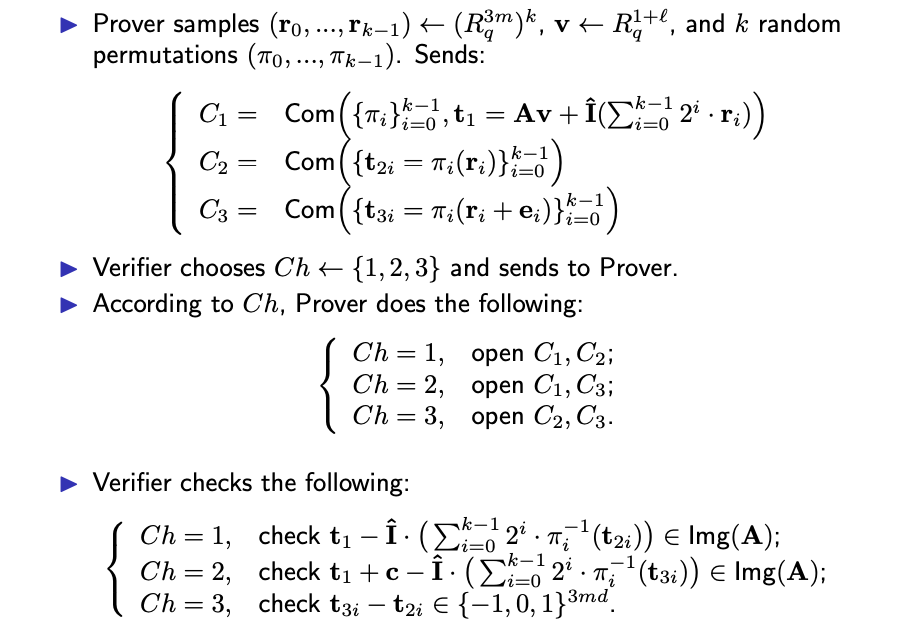
\includegraphics[scale=0.65]{14.png}
	\end{minipage}
\end{frame}







\end{document}

%%%%%%%%%%%%%%%%%%%%%%%%%%%%%%%%%%%%%%%%%%%%%%%%%%%%%%%%%%%%%%\\
%\begin{frame}{Sketch of proof}
%	\begin{minipage}{0.45\linewidth}
%		\begin{figure}[H]
%			%	\small
%			\centering
%			\begin{tikzpicture}
%			%%%%%%%%%%%%%%%%%%%%%%%%%%%%%%%%%%%%%%%%%%%%%%%%%%%%%%%Header Line
%			\node at (0.8,0) {1};
%			\node at (1.5,0) {$\dots$};
%			\node at (2.4,0) {$i$};
%			\node at (3.1,0) {$\dots$};
%			\node at (3.8,0) {$j$};
%			\node at (4.5,0) {$\dots$};
%			\node at (5.2,0) {$n$};
%			\draw [line width=0.25mm,-] (0.3,-0.3) --(6,-0.3) node[right]{$P$};
%			%	%%%%%%%%%%%%%%%%%%%%%%%%%%%%%%%%%%%%%%%%%%%%%%%%%%%%%%%dots Line
%			\draw[line width=0.35mm,loosely dotted] (0.8,-0.5)-- (0.8,-2.5);
%			\draw[line width=0.35mm,loosely dotted] (1.5,-0.5)-- (1.5,-2.5);
%			\draw[line width=0.35mm,loosely dotted] (2.4,-.5)-- (2.4,-0.9);
%			\draw[line width=0.35mm,loosely dotted] (2.4,-1.55)-- (2.4,-2.5);
%			\draw[line width=0.35mm,loosely dotted] (3.1,-.5)-- (3.1,-2.5);
%			\draw[line width=0.35mm,loosely dotted] (3.8,-.5)-- (3.8,-2);
%			\draw[line width=0.35mm,loosely dotted] (4.5,-.5)-- (4.5,-2.5);
%			\draw[line width=0.35mm,loosely dotted] (5.2,-.5)-- (5.2,-2.5);
%			%%%%%%%%%%%%%%%%%%%%%%%%%%%%%%%%%%%%%%%%%%%%%%%%%%%%%%% Braces
%			\draw[decoration={brace,raise=5pt},decorate] (2.4,-2.55) -- node[left=5pt] {\scriptsize$x$-1} (2.4,-1.47);
%			%	\draw[decoration={brace,raise=5pt},decorate] (5,-2.55) -- node[left=5pt] {$k$} (5,-1.8);
%			%%%%%%%%%%%%%%%%%%%%%%%%%%%%%%%%%%%%%%%%%%%%%%%%%%%%%%%	
%			\node at (2.4,-1.2) {$j$};
%			\node at (3.8,-2.25) {$i$};
%			%%%%%%%%%%%%%%%%%%%%%%%%%%%%%%%%%%%%%%%%%%%%%%%%%%%%%%%Identiti Numbers
%			\node at (0.8,-2.7) {1};
%			\node at (1.5,-2.7) {$\dots$};
%			\node at (2.4,-2.7) {$i$};
%			\node at (3.1,-2.7) {$\dots$};
%			\node at (3.8,-2.7) {$j$};
%			\node at (4.5,-2.7) {$\dots$};
%			\node at (5.2,-2.7) {$n$};
%			%%%%%%%%%%%%%%%%%%%%%%%%%%%%%%%%%%%%%%%%%%%%%%%%%%%%%%%	
%			\node at (0.8,-3.1) {$\vdots$};
%			\node at (1.5,-3.1) {$\vdots$};
%			\node at (2.4,-3.1) {$\vdots$};
%			\node at (3.1,-3.1) {$\vdots$};
%			\node at (3.8,-3.1) {$\vdots$};
%			\node at (4.5,-3.1) {$\vdots$};
%			\node at (5.2,-3.1) {$\vdots$};	
%			%%%%%%%%%%%%%%%%%%%%%%%%%%%%%%%%%%%%%%%%%%%%%%%%%%%%%%%	
%			\draw [line width=0.3mm,-,orange] (0.3,-2.65)node[left]{$\mu^{ij}$} -- (2.2,-2.65) -- (2.4,-1.3) -- (2.4,-1.3) -- (2.6,-2.65)-- (3.6,-2.65) -- (3.8,-2.33)-- (3.8,-2.33) -- (4,-2.65) -- (5.8,-2.65);
%			\draw [line width=0.3mm,-,blue] (0.5,-2.75) -- (6,-2.75)node[right]{$\mu^{I}$};
%			\end{tikzpicture}
%			\caption*{ one-couple matching $\mu^{ij}$ length $(x,1)$.}
%			\label{Fig2}
%		\end{figure}
%	\end{minipage}~~~~~~~~~~~~~~~~~~~~~~~~~
%	\begin{minipage}{0.45\linewidth}
%		\begin{figure}[H]
%			\centering
%			\begin{tikzpicture}
%			%%%%%%%%%%%%%%%%%%%%%%%%%%%%%%%%%%%%%%%%%%%%%%%%%%%%%%%Header Line
%			%	\node at (1.5,0) {1};
%			%	\node at (2.5,0) {$2$};
%			%	%	\node at (4.5,0) {$\dots$};
%			%	\node at (6,0) {$n$};
%			%	\draw [line width=0.25mm,-] (0.7,-0.3)-- (7,-.3) node[right]{$P$};
%			%	%%%%%%%%%%%%%%%%%%%%%%%%%%%%%%%%%%%%%%%%%%%%%%%%%%%%%%%dots Line
%			\draw[line width=0.35mm] (1.5,-0.5)-- (1.5,-2.6);
%			\draw[line width=0.35mm] (2.5,-2)-- (2.5,-2.6);
%			\draw[decoration={brace,raise=5pt},decorate] (1.5,-.5) -- node[right=5pt] {$x$} (1.5,-2.6);
%			\draw[decoration={brace,raise=5pt},decorate] (2.5,-2) -- node[right=5pt] {$1$} (2.5,-2.6);
%			%	\draw[line width=0.35mm,loosely dotted] (3.5,-0.5)-- (3.5,-2.85);
%			%	\draw[line width=0.35mm,loosely dotted] (2.5,-0.5)-- (2.5,-2.85);
%			%	\draw[line width=0.35mm,loosely dotted] (4.5,-0.5)-- (4.5,-2.85);
%			%	\draw[line width=0.35mm,loosely dotted] (6,-0.5)-- (6,-2.85);
%			%%%%%%%%%%%%%%%%%%%%%%%%%%%%%%%%%%%%%%%%%%%%%%%%%%%%%%%Identiti Numbers
%			%	\draw [line width=0.3mm,-,cyan] (0.7,-1) --(7.3,-1)node[right]{$\bar{{\mu}}$};
%			%	\draw [line width=0.3mm,-,green] (0.7,-2.5) -- (7.3,-2.5)node[right]{$\mu$};
%			%	\draw [line width=0.3mm,-,orange] (0.4,-1.15)node[left]{$\mu^S$}-- (2.5,-1.15)--(2.7,-2.35)--(7,-2.35);
%			%	\draw [line width=0.3mm,-,red] (0.4,-2.35)node[left]{$\mu^{\bar{S}}$} --	\NoNumber{} (2.5,-2.35)--(2.7,-1.15)--(7,-1.15);
%			\end{tikzpicture}
%			\caption*{$\alpha_{x1}$ is the same...}
%		\end{figure}
%	\end{minipage}
%\end{frame}
%%%%%%%%%%%%%%%%%%%%%%%%%%%%%%%%%%%%%%%%%%%%%%%%%%%%%%%%%%%%%%%
%\begin{frame}{Sketch of proof}
%	\begin{figure}
%		\centering
%		\begin{tikzpicture}
%		%%%%%%%%%%%%%%%%%%%%%%%%%%%%%%%%%%%%%%%%%%%%%%%%%%%%%%%Header Line
%		\node at (0.8,0) {1};
%		\node at (1.5,0) {$\dots$};
%		\node at (2.4,0) {$i$};
%		\node at (3.1,0) {$\dots$};
%		\node at (4,0) {$j$};
%		\node at (4.7,0) {$\dots$};
%		\node at (5.4,0) {$n$};
%		\draw [line width=0.25mm,-] (0.3,-0.3) -- (6,-0.3) node[right]{$P$};
%		%	%%%%%%%%%%%%%%%%%%%%%%%%%%%%%%%%%%%%%%%%%%%%%%%%%%%%%%%dots Line
%		\draw[line width=0.35mm,loosely dotted] (0.8,-0.5)-- (0.8,-2.5);
%		%	\draw[line width=0.4mm,loosely dotted] (1.8,-0.5)-- (1.8,-2.4);
%		\draw[line width=0.35mm,loosely dotted] (1.5,-0.5)-- (1.5,-2.5);
%		%	\draw[line width=0.4mm,loosely dotted] (2.2,-0.5)-- (2.2,-2.4);
%		\draw[line width=0.35mm,loosely dotted] (2.4,-.5)-- (2.4,-0.9);
%		\draw[line width=0.35mm,loosely dotted] (2.4,-1.55)-- (2.4,-2.5);
%		\draw[line width=0.35mm,loosely dotted] (3.1,-.5)-- (3.1,-2.5);
%		\draw[line width=0.35mm,loosely dotted] (4,-.5)-- (4,-1.2);
%		\draw[line width=0.35mm,loosely dotted] (4,-1.9)-- (4,-2.5);
%		\draw[line width=0.35mm,loosely dotted] (4.7,-.5)-- (4.7,-2.5);
%		\draw[line width=0.35mm,loosely dotted] (5.4,-.5)-- (5.4,-2.5);
%		%%%%%%%%%%%%%%%%%%%%%%%%%%%%%%%%%%%%%%%%%%%%%%%%%%%%%%% Braces
%		\draw[decoration={brace,raise=5pt},decorate] (2.4,-2.55) -- node[left=5pt] {\scriptsize$x$-1} (2.4,-1.47);
%		%	\draw[decoration={brace,raise=5pt},decorate] (5,-2.55) -- node[left=5pt] {$k$} (5,-1.8);
%		%%%%%%%%%%%%%%%%%%%%%%%%%%%%%%%%%%%%%%%%%%%%%%%%%%%%%%%	
%		\node at (2.4,-1.2) {$j$};
%		\node at (4,-1.4 ) {$i$};
%		%%%%%%%%%%%%%%%%%%%%%%%%%%%%%%%%%%%%%%%%%%%%%%%%%%%%%%%Identiti Numbers
%		\node at (0.8,-2.7) {1};
%		\node at (1.5,-2.7) {$\dots$};
%		\node at (2.4,-2.7) {$i$};
%		\node at (3.1,-2.7) {$\dots$};
%		\node at (4,-2.7) {$j$};
%		\node at (4.7,-2.7) {$\dots$};
%		\node at (5.4,-2.7) {$n$};
%		%%%%%%%%%%%%%%%%%%%%%%%%%%%%%%%%%%%%%%%%%%%%%%%%%%%%%%%	
%		\node at (0.8,-3.1) {$\vdots$};
%		\node at (1.5,-3.1) {$\vdots$};
%		\node at (2.4,-3.1) {$\vdots$};
%		\node at (3.1,-3.1) {$\vdots$};
%		\node at (4,-3.1) {$\vdots$};
%		\node at (4.7,-3.1) {$\vdots$};
%		\node at (5.4,-3.1) {$\vdots$};	
%		%%%%%%%%%%%%%%%%%%%%%%%%%%%%%%%%%%%%%%%%%%%%%%%%%%%%%%%	
%		\draw [line width=0.3mm,-,orange] (0.3,-2.65) node[left]{$\mu^{ij}$}(0.3,-2.65)--(2.2,-2.65)--(2.4,-1.3) -- (2.6,-2.65) -- (3.8,-2.65)-- (4,-1.5)  -- (4.2,-2.65)   -- (5.8,-2.65);
%		\draw [line width=0.3mm,-,blue] (0.5,-2.75) -- (6,-2.75)node[right]{$\mu^{I}$};
%		%\draw[decoration={brace,raise=5pt},decorate] (2,-2.4) -- node[left=5pt] {\small$x$-$1$} (2,-1.3);
%		\draw[decoration={brace,raise=5pt},decorate] (4,-2.4) -- node[left=5pt] {\scriptsize$y$-1} (4,-1.7);
%		\end{tikzpicture}
%		\caption*{A one-couple matching $\mu^{ij}$ of length $(x,y)$.}
%		\label{extraFig}
%	\end{figure}
%\end{frame}
%%%%%%%%%%%%%%%%%%%%%%%%%%%%%%%%%%%%%%%%%%%%%%%%%%%%%%%%%%%%%%%\\
%\begin{frame}
%	\begin{minipage}{.45\linewidth}
%		\begin{figure}[H]
%			\centering
%			\begin{tikzpicture}
%			%%%%%%%%%%%%%%%%%%%%%%%%%%%%%%%%%%%%%%%%%%%%%%%%%%%%%%%Header Line
%			%	\node at (1.5,0) {1};
%			%	\node at (2.5,0) {$2$};
%			%	%	\node at (4.5,0) {$\dots$};
%			%	\node at (6,0) {$n$};
%			%	\draw [line width=0.25mm,-] (0.7,-0.3)-- (7,-.3) node[right]{$P$};
%			%	%%%%%%%%%%%%%%%%%%%%%%%%%%%%%%%%%%%%%%%%%%%%%%%%%%%%%%%dots Line
%			\draw[line width=0.35mm] (1.5,-0.5)-- (1.5,-2.6);
%			\draw[line width=0.35mm] (2.5,-1)-- (2.5,-2.6);
%			\draw[line width=0.35mm] (3.5,-2)-- (3.5,-2.6);
%			\draw[line width=0.35mm] (4.5,-2)-- (4.5,-2.6);
%			\draw[decoration={brace,raise=5pt},decorate] (1.5,-.5) -- node[right=5pt] {$x$} (1.5,-2.6);
%			\draw[decoration={brace,raise=5pt},decorate] (2.5,-1) -- node[right=5pt] {$y$} (2.5,-2.6);
%			\draw[decoration={brace,raise=5pt},decorate] (3.5,-2) -- node[right=5pt] {$1$} (3.5,-2.6);
%			\draw[decoration={brace,raise=5pt},decorate] (4.5,-2) -- node[right=5pt] {$1$} (4.5,-2.6);
%			%	\draw[line width=0.35mm,loosely dotted] (3.5,-0.5)-- (3.5,-2.85);
%			%	\draw[line width=0.35mm,loosely dotted] (2.5,-0.5)-- (2.5,-2.85);
%			%	\draw[line width=0.35mm,loosely dotted] (4.5,-0.5)-- (4.5,-2.85);
%			%	\draw[line width=0.35mm,loosely dotted] (6,-0.5)-- (6,-2.85);
%			%%%%%%%%%%%%%%%%%%%%%%%%%%%%%%%%%%%%%%%%%%%%%%%%%%%%%%%Identiti Numbers
%			%	\draw [line width=0.3mm,-,cyan] (0.7,-1) --(7.3,-1)node[right]{$\bar{{\mu}}$};
%			%	\draw [line width=0.3mm,-,green] (0.7,-2.5) -- (7.3,-2.5)node[right]{$\mu$};
%			%	\draw [line width=0.3mm,-,orange] (0.4,-1.15)node[left]{$\mu^S$}-- (2.5,-1.15)--(2.7,-2.35)--(7,-2.35);
%			%	\draw [line width=0.3mm,-,red] (0.4,-2.35)node[left]{$\mu^{\bar{S}}$} -- (2.5,-2.35)--(2.7,-1.15)--(7,-1.15);
%			\end{tikzpicture}
%			\caption*{$\alpha_{xy}+\alpha_{11}$}
%		\end{figure}
%	\end{minipage} {\Huge=}
%	\begin{minipage}{.45\linewidth}
%		\begin{figure}[H]
%			\centering
%			\begin{tikzpicture}
%			%%%%%%%%%%%%%%%%%%%%%%%%%%%%%%%%%%%%%%%%%%%%%%%%%%%%%%%Header Line
%			%	\node at (1.5,0) {1};
%			%	\node at (2.5,0) {$2$};
%			%	%	\node at (4.5,0) {$\dots$};
%			%	\node at (6,0) {$n$};
%			%	\draw [line width=0.25mm,-] (0.7,-0.3)-- (7,-.3) node[right]{$P$};
%			%	%%%%%%%%%%%%%%%%%%%%%%%%%%%%%%%%%%%%%%%%%%%%%%%%%%%%%%%dots Line
%			\draw[line width=0.35mm] (1.5,-0.5)-- (1.5,-2.6);
%			\draw[line width=0.35mm] (3.5,-1)-- (3.5,-2.6);
%			\draw[line width=0.35mm] (2.5,-2)-- (2.5,-2.6);
%			\draw[line width=0.35mm] (4.5,-2)-- (4.5,-2.6);
%			\draw[decoration={brace,raise=5pt},decorate] (1.5,-.5) -- node[right=5pt] {$x$} (1.5,-2.6);
%			\draw[decoration={brace,raise=5pt},decorate] (3.5,-1) -- node[right=5pt] {$y$} (3.5,-2.6);
%			\draw[decoration={brace,raise=5pt},decorate] (2.5,-2) -- node[right=5pt] {$1$} (2.5,-2.6);
%			\draw[decoration={brace,raise=5pt},decorate] (4.5,-2) -- node[right=5pt] {$1$} (4.5,-2.6);
%			\end{tikzpicture}
%			\caption*{$\alpha_{x1}+ \alpha_{y1}$}
%		\end{figure}
%	\end{minipage}
%\end{frame}
%%%%%%%%%%%%%%%%%%%%%%%%%%%%%%%%%%%%%%%%%%%%%%%%%%%%%%%%%%%%%%%\\
%\begin{frame}
%	\begin{figure}[H]
%		\centering
%		\begin{tikzpicture}
%		\draw[line width=0.35mm] (1.5,-0.5)-- (1.5,-2.6);
%		\draw[line width=0.35mm] (2.5,-0.5)-- (2.5,-2.6);
%		\draw[decoration={brace,raise=5pt},decorate] (1.5,-.5) -- node[right=5pt] {$x$} (1.5,-2.6);
%		\draw[decoration={brace,raise=5pt},decorate] (2.5,-.5) -- node[right=5pt] {$x$} (2.5,-2.6);
%		\end{tikzpicture}
%		\caption*{$\alpha_{xx}= $ something fix for every $x$.}
%	\end{figure}
%	
%	Therefore,
%	\begin{align*}
%	&\alpha_{x1}, \text{is the same} \\
%	&\alpha_{xy}=\alpha_{x1}+\alpha_{y1}-\alpha_{11} \\
%	&\alpha_{xx}= 2 \alpha_{x1} - \alpha_{11}
%	\end{align*}
%\end{frame}
%
%%%%%%%%%%%%%%%%%%%%%%%%%%%%%%%%%%%%%%%%%%%%%%%%%%%%%%%%%%%%%%%
%\begin{frame}
%	\begin{definition} \label{def:pri} \rm
%		A {\it priority assignment rule} $\pi$ is a collection of maps ${\pi}^{k+1} : \Sigma^k \rightarrow M$ with $k\in \{0,1,\dots,n-1\}$ such that $\pi ^{k+1}(\sigma^k[M]) \notin \sigma^k[M]$, for all $\sigma^k \in \Sigma^k$ and all $k$. 
%	\end{definition}
%	\begin{definition} \label{def:option} \rm  
%		An {\it option-set assignment rule} $\lambda$ is a collection of maps ${\lambda}^{k+1} : \Sigma^k \rightarrow 2^{W \cup \emptyset}$ with  $k\in \{0,1 \ldots, n-1\}$
%		satisfying the following conditions:
%		\begin{enumerate}
%			\item [i.] $\lambda ^{k+1} (\sigma^k) \subset (W \cup \emptyset) \setminus \{\sigma^k[W]\}$ for all $\sigma^k\in \Sigma^k$ and $k$.
%			\item [ii.]  If either $\emptyset \in \sigma^k[W]$ or $w_{j^*} \in \sigma^k[W]$, then $\lambda^{k+1}(\sigma^k) = \emptyset$. 
%			\item [iii.] If $\lambda^{k+1}(\sigma^{k}) \neq \emptyset$, then $w_{j^*} \in \lambda^{k+1} (\sigma^{k})$ for all $\sigma^k \in \Sigma^k$ and $k$.
%		\end{enumerate}
%	\end{definition}
%\end{frame}
